\documentclass[10pt,a4paper]{article}
\usepackage[utf8]{inputenc}
\usepackage[spanish]{babel}
\usepackage{amsmath}
\usepackage{amsfonts}
\usepackage{amssymb}
\usepackage{makeidx}
\usepackage{graphicx}
\usepackage{lmodern}
\usepackage{kpfonts}
\usepackage[left=2cm,right=2cm,top=2cm,bottom=2cm]{geometry}
\begin{document}
\begin{center}

\includegraphics[scale=0.2]{imagenes/upzmg.png} 
\end{center}
\large \huge\textbf{  Descripcion de condiciones de singularidad de manipuladores seriales  }\\ \\\begin{large}

\end{large}
\large \begin{Large}
Un robot manipulador serie es una cadena cinematica abierto
ta compuesta de una secuencia de elementos estructurales riıgidos, denominados eslabones, conectados entre si a traves de articulaciones, que permiten el movimiento relativo de cada par
de eslabones consecutivos. Al final del ultimo eslabon puede anadirse una herramienta o dispositivo, denominado elemento terminal.

\end{Large}
\begin{Large}
La posicion y orientacion del elemento terminal (pose) puede expresarse mediante una funcion diferenciable f : \textbf{C → X}
en donde C es el espacio de las variables articulares, denominado espacio de configuraciones y X es el espacio de todas las
posiciones y orientaciones del elemento terminal con respecto a un cierto sistema de referencia, denominado espacio cartesiano. \\ \\ \\
 Asimismo, a cada articulacion  se le asocia un sistema de coordenadas {i} que se utiliza para describir su posicion y orientacion relativas. La relacion entre los sistemas de coordenadas asociados a articulaciones consecutivas viene descrita
mediante una matriz de transformacion homog ´ enea construida a partir de los parametros de \textbf{Denavit-Hartenberg} \\ \\ 
un sistema de coordenadas ortonormal (oi,xi,yi,zi) una matriz de transformacion homogenea que relaciona dicho sistema de coordenadas con el anterior (el sistema de coordenadas de la
primera articulacion se relaciona con el sistema de referencia del mundo, representado por {0}).
\end{Large}
\begin{center}
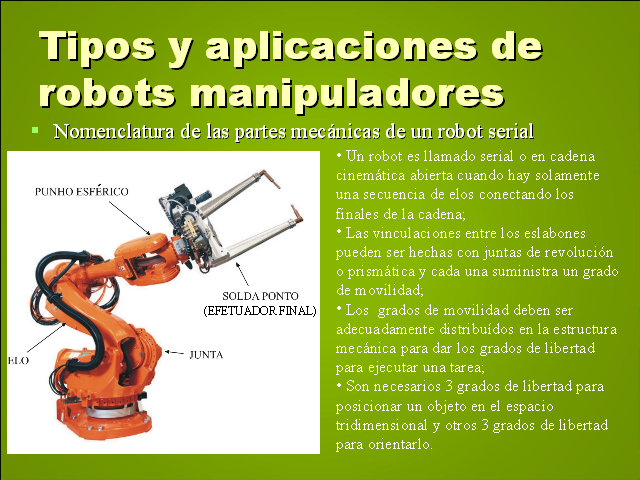
\includegraphics[scale=0.7]{imagenes/brazo.png} 
\end{center}
\begin{Large}
El propósito de este índice es medir la capacidad de un
robot, en cierta configuración, para generar velocidades en el
efector final. Este índice de desempeño es proporcional al volumen del elipsoide de velocidad.  Para el caso general (incluyendo robots redundantes) la manipulabilidad esta definida de la
siguiente manera:
w = A/det(jJr) (3)
Para robots no redundantes se tiene que w = | det(J)| . La
manipulabilidad es equivalente al producto de los valores singulares, w = <xi<x2 • • • cr \\ \\
Para que los índices de desempeño basados en la matriz Jacobiana puedan ser evaluados de manera consistente, los elementos de la matriz Jacobiana deben ser dimensionalmente homogéneos (Lipkin, 1989)
\end{Large}
\begin{center}
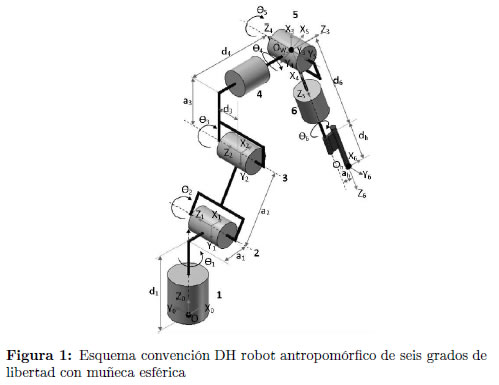
\includegraphics[scale=0.8]{imagenes/brazo 2.jpg} 
\end{center}
\large \huge \textbf{•REFENECIAS} \\

{@article{saravia2009revision,
  title={Revisi{\'o}n del estado del arte de manipuladores paralelos},
  author={Saravia, Darly Babeth P and Lopez, Marlon Jhair H and Riaza, Hector Fabio Q},
  journal={Scientia et technica},
  volume={2},
  number={42},
  pages={81--86},
  year={2009},
  publisher={Universidad Tecnol{\'o}gica de Pereira}}
}
\end{document}